\documentclass[12pt]{article}
\usepackage{lingmacros}
\usepackage{tree-dvips}
\usepackage{url}

\usepackage{pgfplotstable}
\usepackage{pgfplots}
\pgfplotsset{compat = 1.3}
\usepackage{subfig}

\usepackage{amssymb}
\setcounter{tocdepth}{3}
\usepackage{graphicx}

\usepackage{times}
\usepackage{graphicx}
\usepackage{latexsym}
\usepackage{algorithm}
\usepackage{float}
\usepackage[noend]{algpseudocode}
\usepackage{amssymb}
\usepackage{amsmath,amsthm} 
\usepackage{amsfonts}
%%%%%%%\usepackage{mathtools}
\usepackage{verbatim} 
\usepackage{longtable}
\usepackage{graphicx}
\usepackage{booktabs}
\usepackage{epstopdf}
\usepackage{longtable}
\usepackage{pgfpages}
\usepackage{multirow}
\usepackage{varwidth}
%\usepackage{tabularx} % for aligning & numbering equations on the same line
%\usepackage{enumitem}
\usepackage{pifont}

\newcommand{\oled}{\textsf{OLED}}
\newcommand{\home}{\texttt{/oledhome}}

\title{\oled \  User Manual}
%\date{}

\begin{document}

\maketitle

\section{Installation}

\begin{itemize}
\item Clone of download the source code from \url{https://github.com/nkatzz/OLED}. 
\item Open a terminal and navigate to the location where the source code is cloned. In what follows we'll refer to this directory by \home.
\item From inside \home \ type in the terminal: \\ \texttt{cp -r OLED/install-scripts .}\\
Your \home \ should now look like this:

\begin{figure}[h]
\centering
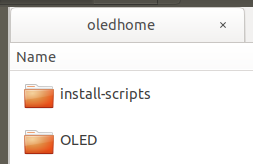
\includegraphics[width=0.2\textwidth]{./figures/oledhome-1}
\label{fig:oled_schema}
\end{figure}  

\item cd into the install-scripts and type:\\
\texttt{./install.sh}\\
You will need sudo priviledges to run the install script. The whole process will take some time to complete.
\item If all goes well your \home \ should now look like this:\\
ADD A SCREENSHOT
\item Modify paths.

\end{itemize}


\subsection*{Parsing CAVIAR Into Mongo}
\begin{itemize}
\item Download the dataset from here: \scriptsize
 \url{http://users.iit.demokritos.gr/~nkatz/data/CAVIAR-abrupt-original.tar.gz} \normalsize 
\item Run: \\
\scriptsize \texttt{java -cp oled.jar:/lib/jep-3.6.3.jar -Djava.library.path=/opt/jep-home/lib/python/jep data\_handling.ParseCAVIAR /path/to/unzipped.dataset dbname} \normalsize \\
For example: \\
\scriptsize \texttt{java -cp oled.jar:/lib/jep-3.6.3.jar -Djava.library.path=/opt/jep-home/lib/python/jep data\_handling.ParseCAVIAR /home/nkatz/dev/CAVIAR-abrupt-original caviar} \normalsize
\end{itemize}

\subsection*{Building LoMRF}
Run sbt from within the \texttt{auxlib} folder and do \texttt{publishLocal}. Then run sbt from within the LoMRF folder and do \texttt{publishLocal}.

\subsection*{\texttt{.profile}}
\begin{figure*}[h]
\centering
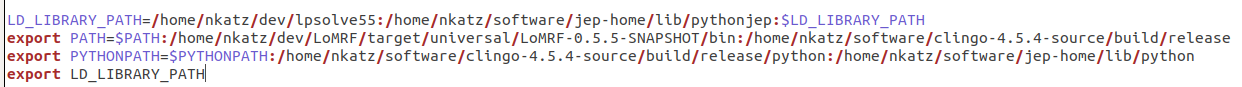
\includegraphics[width=\textwidth]{./figures/profile-example.png}
\end{figure*} 

\end{document}
